%第3章


\section{要求定義}


商品識別システムがどのように機能すべきかという振る舞いと,その外部環境を表すためにユースケース図を作成した.以下に最初に作成した図\ref{usecase1}を載せる.

図\ref{usecase1}においてユースケースとしてはカートの登録,商品をカートに入れる,カートでゲートを通る,QRコードを読み取り決済するの4つとした.入退店の管理をカートの登録とカートでゲートを通るの2つのユースケースで行おうと設計したが,簡単に決済まで行えるという前提から,ユースケースの数が少ないほうが手順が減り簡単という条件により適すると考え,ユースケースを統合し全体のユースケース数を削減した.

ユースケースを統合しユースケースの数を減らしたユースケース図は図\ref{usecase2}に示す.

\begin{figure}[htbp]
\centering
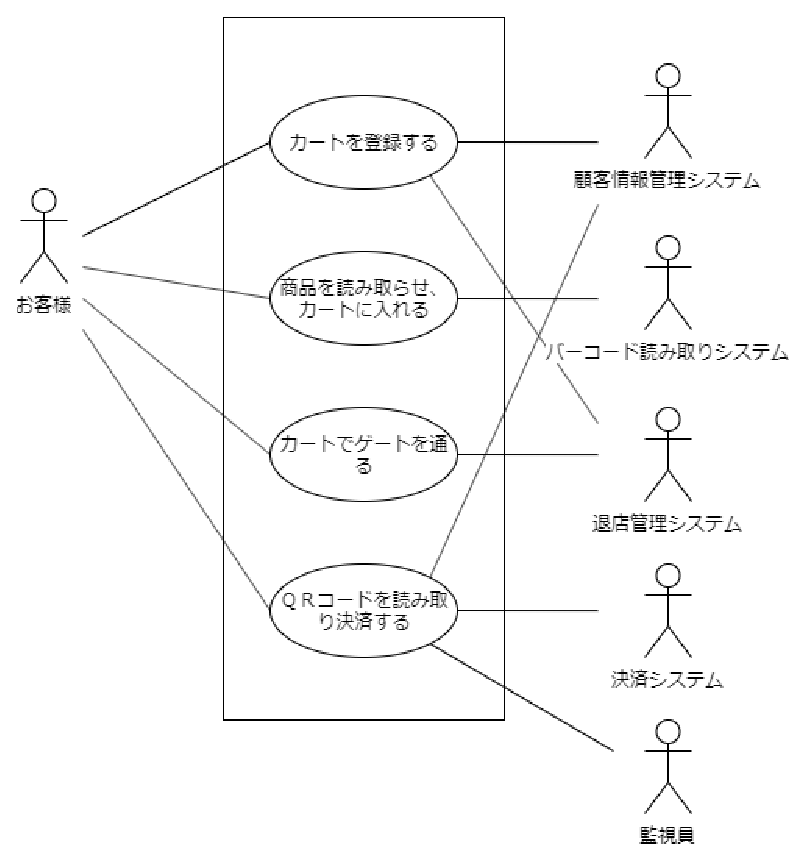
\includegraphics[width = 9cm]{./picture/usecase1.eps}
\caption{ユースケース図(1)}
\label{usecase1}
\end{figure}

\begin{figure}[htbp]
\centering
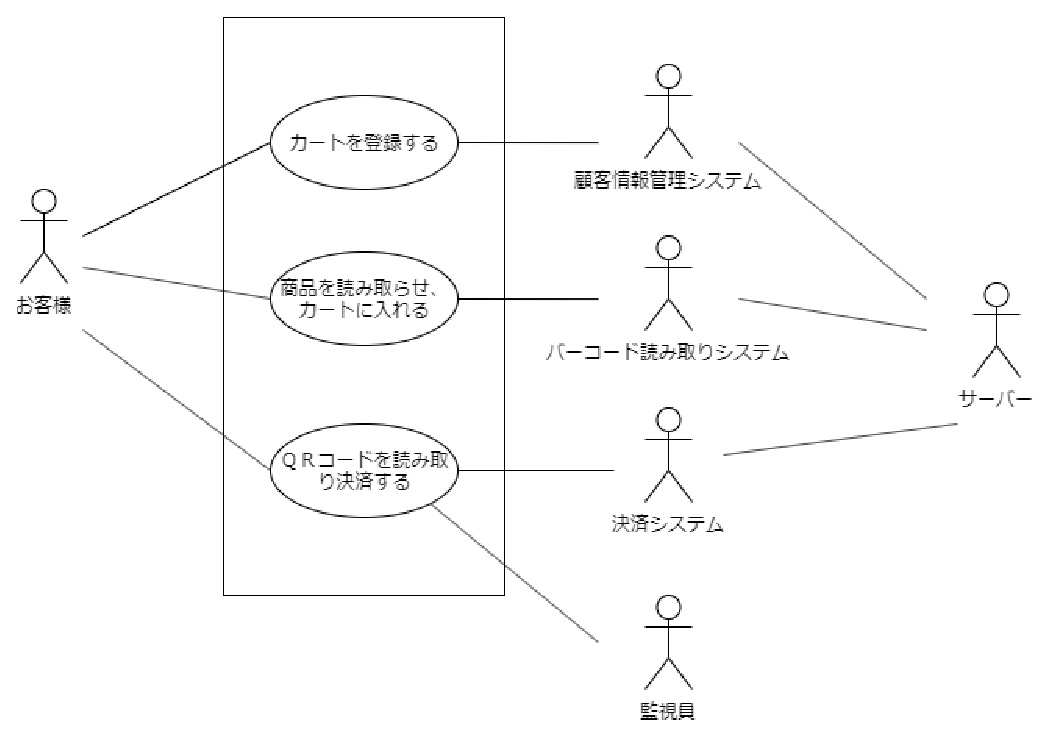
\includegraphics[width = 9cm]{./picture/usecase2.eps}
\caption{ユースケース図(2)}
\label{usecase2}
\end{figure}

\begin{figure}[htbp]
\centering
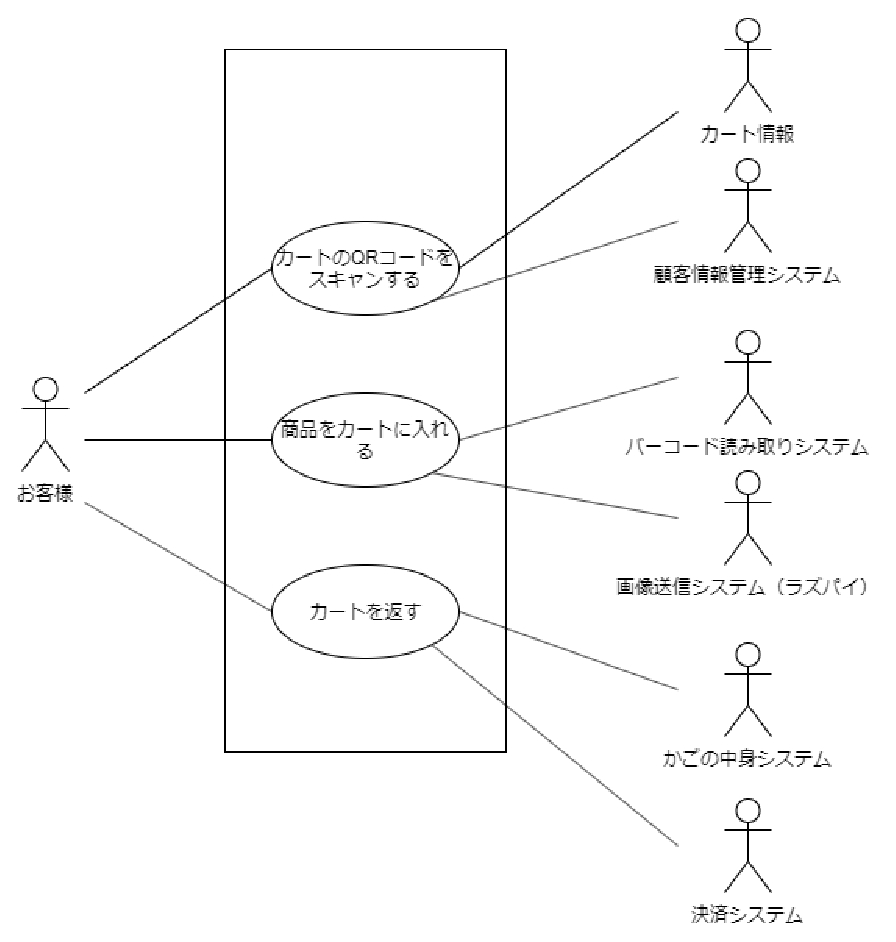
\includegraphics{./picture/usecase3.eps}
\caption{システムのユースケース図(3)}
\label{usecase3}
\end{figure}

\begin{figure}[htbp]
\centering
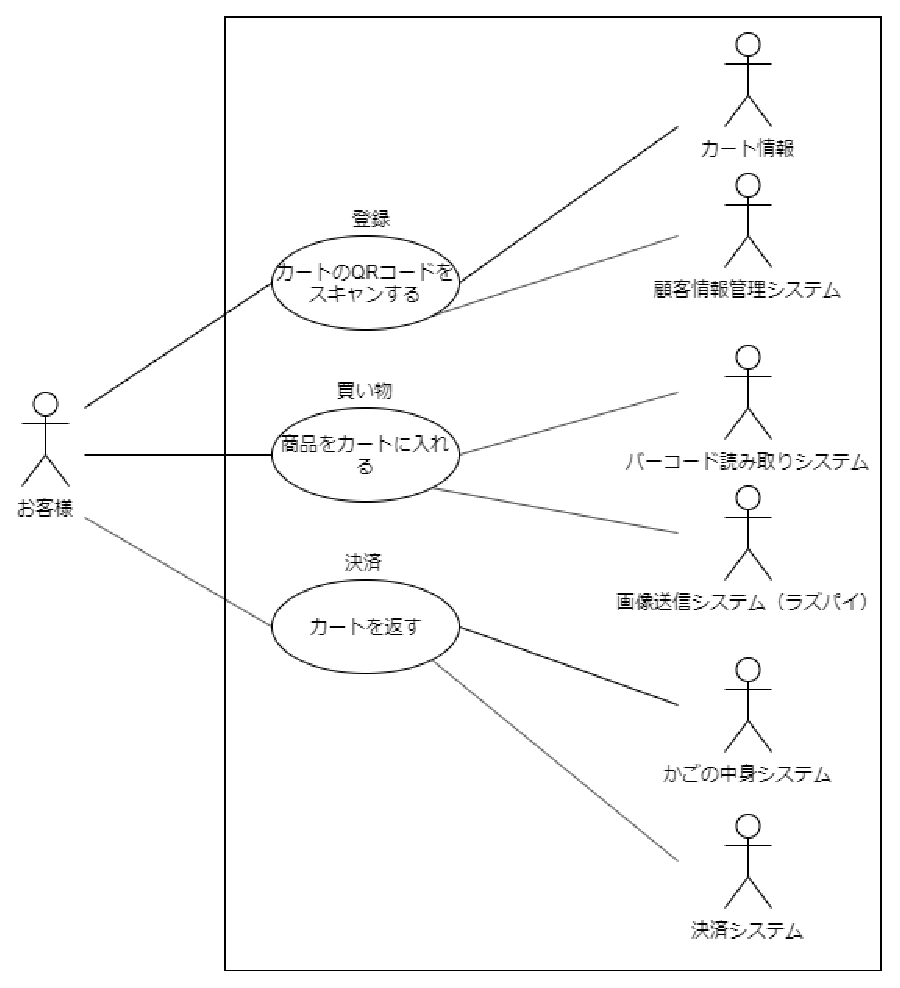
\includegraphics[width = 15cm]{./picture/usecase_qr.eps}
\caption{QRコードを用いたシステムのユースケース図}
\label{usecase_qr}
\end{figure}

\begin{figure}[htbp]
\centering
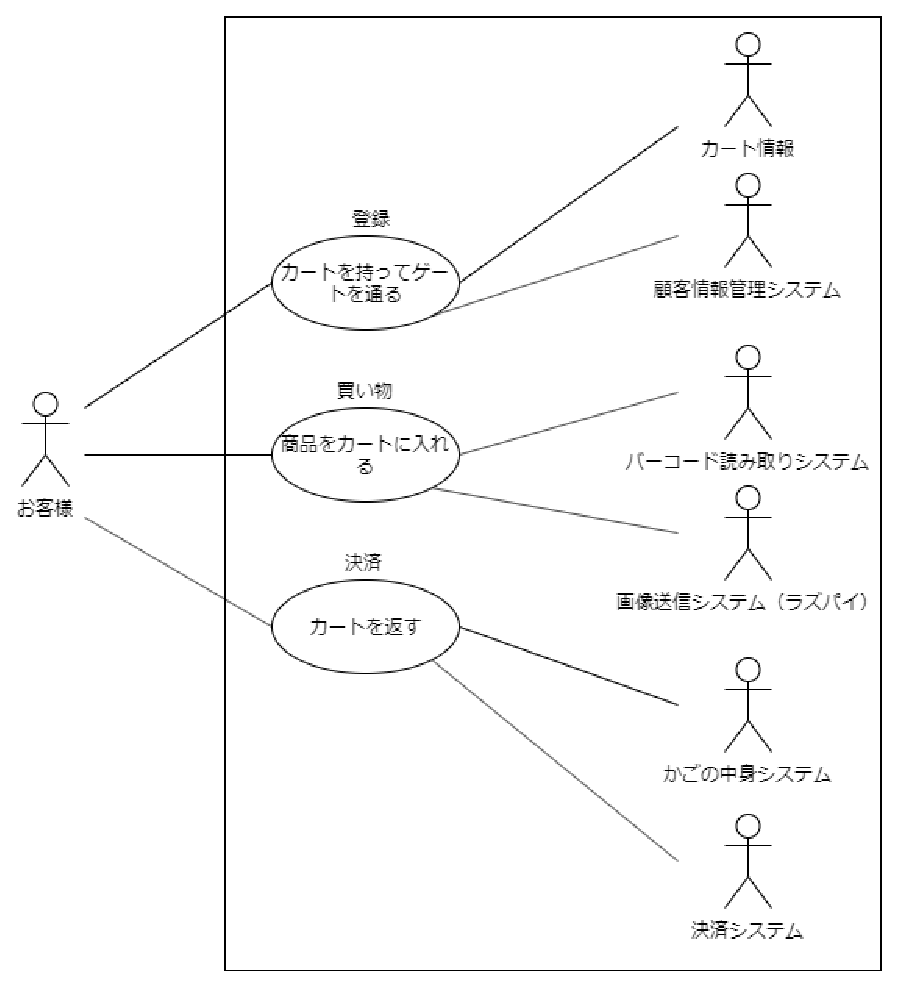
\includegraphics[width = 15cm]{./picture/usecase_ic.eps}
\caption{ICタグを用いたシステムのユースケース図}
\label{usecase_ic}
\end{figure}


